\documentclass[]{book}
\usepackage{lmodern}
\usepackage{amssymb,amsmath}
\usepackage{ifxetex,ifluatex}
\usepackage{fixltx2e} % provides \textsubscript
\ifnum 0\ifxetex 1\fi\ifluatex 1\fi=0 % if pdftex
  \usepackage[T1]{fontenc}
  \usepackage[utf8]{inputenc}
\else % if luatex or xelatex
  \ifxetex
    \usepackage{mathspec}
  \else
    \usepackage{fontspec}
  \fi
  \defaultfontfeatures{Ligatures=TeX,Scale=MatchLowercase}
\fi
% use upquote if available, for straight quotes in verbatim environments
\IfFileExists{upquote.sty}{\usepackage{upquote}}{}
% use microtype if available
\IfFileExists{microtype.sty}{%
\usepackage{microtype}
\UseMicrotypeSet[protrusion]{basicmath} % disable protrusion for tt fonts
}{}
\usepackage[margin=1in]{geometry}
\usepackage{hyperref}
\hypersetup{unicode=true,
            pdftitle={Linguistic Geocomputation with R},
            pdfauthor={George Moroz},
            pdfborder={0 0 0},
            breaklinks=true}
\urlstyle{same}  % don't use monospace font for urls
\usepackage{natbib}
\bibliographystyle{apalike}
\usepackage{color}
\usepackage{fancyvrb}
\newcommand{\VerbBar}{|}
\newcommand{\VERB}{\Verb[commandchars=\\\{\}]}
\DefineVerbatimEnvironment{Highlighting}{Verbatim}{commandchars=\\\{\}}
% Add ',fontsize=\small' for more characters per line
\usepackage{framed}
\definecolor{shadecolor}{RGB}{248,248,248}
\newenvironment{Shaded}{\begin{snugshade}}{\end{snugshade}}
\newcommand{\KeywordTok}[1]{\textcolor[rgb]{0.13,0.29,0.53}{\textbf{#1}}}
\newcommand{\DataTypeTok}[1]{\textcolor[rgb]{0.13,0.29,0.53}{#1}}
\newcommand{\DecValTok}[1]{\textcolor[rgb]{0.00,0.00,0.81}{#1}}
\newcommand{\BaseNTok}[1]{\textcolor[rgb]{0.00,0.00,0.81}{#1}}
\newcommand{\FloatTok}[1]{\textcolor[rgb]{0.00,0.00,0.81}{#1}}
\newcommand{\ConstantTok}[1]{\textcolor[rgb]{0.00,0.00,0.00}{#1}}
\newcommand{\CharTok}[1]{\textcolor[rgb]{0.31,0.60,0.02}{#1}}
\newcommand{\SpecialCharTok}[1]{\textcolor[rgb]{0.00,0.00,0.00}{#1}}
\newcommand{\StringTok}[1]{\textcolor[rgb]{0.31,0.60,0.02}{#1}}
\newcommand{\VerbatimStringTok}[1]{\textcolor[rgb]{0.31,0.60,0.02}{#1}}
\newcommand{\SpecialStringTok}[1]{\textcolor[rgb]{0.31,0.60,0.02}{#1}}
\newcommand{\ImportTok}[1]{#1}
\newcommand{\CommentTok}[1]{\textcolor[rgb]{0.56,0.35,0.01}{\textit{#1}}}
\newcommand{\DocumentationTok}[1]{\textcolor[rgb]{0.56,0.35,0.01}{\textbf{\textit{#1}}}}
\newcommand{\AnnotationTok}[1]{\textcolor[rgb]{0.56,0.35,0.01}{\textbf{\textit{#1}}}}
\newcommand{\CommentVarTok}[1]{\textcolor[rgb]{0.56,0.35,0.01}{\textbf{\textit{#1}}}}
\newcommand{\OtherTok}[1]{\textcolor[rgb]{0.56,0.35,0.01}{#1}}
\newcommand{\FunctionTok}[1]{\textcolor[rgb]{0.00,0.00,0.00}{#1}}
\newcommand{\VariableTok}[1]{\textcolor[rgb]{0.00,0.00,0.00}{#1}}
\newcommand{\ControlFlowTok}[1]{\textcolor[rgb]{0.13,0.29,0.53}{\textbf{#1}}}
\newcommand{\OperatorTok}[1]{\textcolor[rgb]{0.81,0.36,0.00}{\textbf{#1}}}
\newcommand{\BuiltInTok}[1]{#1}
\newcommand{\ExtensionTok}[1]{#1}
\newcommand{\PreprocessorTok}[1]{\textcolor[rgb]{0.56,0.35,0.01}{\textit{#1}}}
\newcommand{\AttributeTok}[1]{\textcolor[rgb]{0.77,0.63,0.00}{#1}}
\newcommand{\RegionMarkerTok}[1]{#1}
\newcommand{\InformationTok}[1]{\textcolor[rgb]{0.56,0.35,0.01}{\textbf{\textit{#1}}}}
\newcommand{\WarningTok}[1]{\textcolor[rgb]{0.56,0.35,0.01}{\textbf{\textit{#1}}}}
\newcommand{\AlertTok}[1]{\textcolor[rgb]{0.94,0.16,0.16}{#1}}
\newcommand{\ErrorTok}[1]{\textcolor[rgb]{0.64,0.00,0.00}{\textbf{#1}}}
\newcommand{\NormalTok}[1]{#1}
\usepackage{longtable,booktabs}
\usepackage{graphicx,grffile}
\makeatletter
\def\maxwidth{\ifdim\Gin@nat@width>\linewidth\linewidth\else\Gin@nat@width\fi}
\def\maxheight{\ifdim\Gin@nat@height>\textheight\textheight\else\Gin@nat@height\fi}
\makeatother
% Scale images if necessary, so that they will not overflow the page
% margins by default, and it is still possible to overwrite the defaults
% using explicit options in \includegraphics[width, height, ...]{}
\setkeys{Gin}{width=\maxwidth,height=\maxheight,keepaspectratio}
\IfFileExists{parskip.sty}{%
\usepackage{parskip}
}{% else
\setlength{\parindent}{0pt}
\setlength{\parskip}{6pt plus 2pt minus 1pt}
}
\setlength{\emergencystretch}{3em}  % prevent overfull lines
\providecommand{\tightlist}{%
  \setlength{\itemsep}{0pt}\setlength{\parskip}{0pt}}
\setcounter{secnumdepth}{5}
% Redefines (sub)paragraphs to behave more like sections
\ifx\paragraph\undefined\else
\let\oldparagraph\paragraph
\renewcommand{\paragraph}[1]{\oldparagraph{#1}\mbox{}}
\fi
\ifx\subparagraph\undefined\else
\let\oldsubparagraph\subparagraph
\renewcommand{\subparagraph}[1]{\oldsubparagraph{#1}\mbox{}}
\fi

%%% Use protect on footnotes to avoid problems with footnotes in titles
\let\rmarkdownfootnote\footnote%
\def\footnote{\protect\rmarkdownfootnote}

%%% Change title format to be more compact
\usepackage{titling}

% Create subtitle command for use in maketitle
\newcommand{\subtitle}[1]{
  \posttitle{
    \begin{center}\large#1\end{center}
    }
}

\setlength{\droptitle}{-2em}
  \title{Linguistic Geocomputation with R}
  \pretitle{\vspace{\droptitle}\centering\huge}
  \posttitle{\par}
  \author{George Moroz}
  \preauthor{\centering\large\emph}
  \postauthor{\par}
  \predate{\centering\large\emph}
  \postdate{\par}
  \date{2018-06-11}

\usepackage{booktabs}
\usepackage{amsthm}
\makeatletter
\def\thm@space@setup{%
  \thm@preskip=8pt plus 2pt minus 4pt
  \thm@postskip=\thm@preskip
}
\makeatother

\usepackage{amsthm}
\newtheorem{theorem}{Theorem}[chapter]
\newtheorem{lemma}{Lemma}[chapter]
\theoremstyle{definition}
\newtheorem{definition}{Definition}[chapter]
\newtheorem{corollary}{Corollary}[chapter]
\newtheorem{proposition}{Proposition}[chapter]
\theoremstyle{definition}
\newtheorem{example}{Example}[chapter]
\theoremstyle{definition}
\newtheorem{exercise}{Exercise}[chapter]
\theoremstyle{remark}
\newtheorem*{remark}{Remark}
\newtheorem*{solution}{Solution}
\begin{document}
\maketitle

{
\setcounter{tocdepth}{1}
\tableofcontents
}
This book is about

\chapter{Introduction}\label{intro}

\section{Why linguistic
geocomputations?}\label{why-linguistic-geocomputations}

\section{Why do we need geostatistics in
linguistics?}\label{why-do-we-need-geostatistics-in-linguistics}

\section{Why R?}\label{why-r}

\chapter{Introduction to R language}\label{introduction-to-r-language}

Since this book includes a lot of R code examples, this chapter will
describe some basics for those, who is not familiar with R. For purposes
of understanding R code in this book you don't need any deep knowledge
of R. In case you want to learn more, there are a lot of good books on
it. I will list only few of them:

\begin{itemize}
\item
\item
\end{itemize}

\section{Instalation}\label{instalation}

\subsection{R instalation}\label{r-instalation}

To download R, go to \href{https://cran.r-project.org/}{CRAN}. Don't try
to pick a mirror that's close to you, instead it is better to use the
cloud mirror, \url{https://cloud.r-project.org}.

\subsection{RStudio}\label{rstudio}

RStudio is an integrated development environment, or IDE, for R
programming. There are two possibilities:

\begin{itemize}
\tightlist
\item
  type R code in the R console pane, and press enter to run it;
\item
  type R code in the Code editor pane, and press Control/Command + Enter
  to run selected part. It is easier to correct and it is possible to
  save the result as a script.
\end{itemize}

\begin{figure}

{\centering 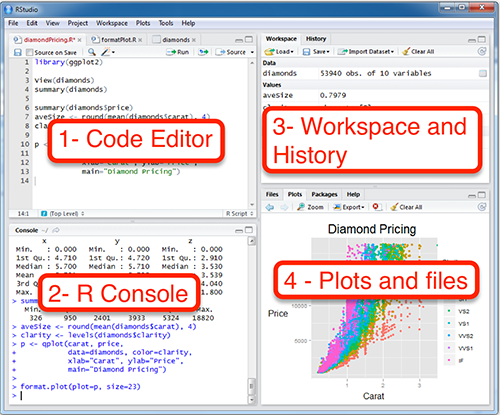
\includegraphics[width=5in]{images/02-rstudio} 

}

\caption{RStudio layout}\label{fig:rstudio}
\end{figure}

When you first launch RStudio it is more likely, that you won't see the
Code Editor pane. It is possible to decrease R Console pane on icons in
the pane's right upper corner.

Everything from this book will be availible without RStudio instalation.
There are a lot of possibilities to work with R not using RStudio such
as R console, command line, Jupyter Notebook, some plugins for working
in Sublime, Vim, Emacs, Atom, Notepad++ and other programming text
editors.

\subsection{RStuio cloud}\label{rstuio-cloud}

It is also possible not to install anything on your own PC, using
\href{https://rstudio.cloud/}{RStudio Cloud}, a web-based interface for
Rstudio and R. In RStudio Cloud it is also possible to share your R
projects and collaborate with a select group in a private space. RStudio
Cloud is currently free to use, but soon there will be free and paid
options.

\section{Base elements, variables, vectors,
dataframe}\label{base-elements-variables-vectors-dataframe}

\subsection{Base elements}\label{base-elements}

\begin{Shaded}
\begin{Highlighting}[]
\DecValTok{7}
\end{Highlighting}
\end{Shaded}

\begin{verbatim}
[1] 7
\end{verbatim}

\begin{Shaded}
\begin{Highlighting}[]
\OperatorTok{-}\FloatTok{5.7}
\end{Highlighting}
\end{Shaded}

\begin{verbatim}
[1] -5.7
\end{verbatim}

\begin{Shaded}
\begin{Highlighting}[]
\StringTok{"bonjour"}
\end{Highlighting}
\end{Shaded}

\begin{verbatim}
[1] "bonjour"
\end{verbatim}

\begin{Shaded}
\begin{Highlighting}[]
\StringTok{"bon mot"}
\end{Highlighting}
\end{Shaded}

\begin{verbatim}
[1] "bon mot"
\end{verbatim}

\begin{Shaded}
\begin{Highlighting}[]
\OtherTok{TRUE}
\end{Highlighting}
\end{Shaded}

\begin{verbatim}
[1] TRUE
\end{verbatim}

\begin{Shaded}
\begin{Highlighting}[]
\OtherTok{FALSE}
\end{Highlighting}
\end{Shaded}

\begin{verbatim}
[1] FALSE
\end{verbatim}

\subsection{Variables}\label{variables}

\begin{Shaded}
\begin{Highlighting}[]
\NormalTok{my_var <-}\StringTok{ }\DecValTok{7}
\NormalTok{my_var}
\end{Highlighting}
\end{Shaded}

\begin{verbatim}
[1] 7
\end{verbatim}

\begin{Shaded}
\begin{Highlighting}[]
\NormalTok{my_var}\OperatorTok{+}\DecValTok{7}
\end{Highlighting}
\end{Shaded}

\begin{verbatim}
[1] 14
\end{verbatim}

\begin{Shaded}
\begin{Highlighting}[]
\NormalTok{my_var}
\end{Highlighting}
\end{Shaded}

\begin{verbatim}
[1] 7
\end{verbatim}

\begin{Shaded}
\begin{Highlighting}[]
\NormalTok{my_var <-}\StringTok{ }\NormalTok{my_var }\OperatorTok{+}\StringTok{ }\DecValTok{7}
\end{Highlighting}
\end{Shaded}

\subsection{Vectors}\label{vectors}

\begin{Shaded}
\begin{Highlighting}[]
\DecValTok{5}\OperatorTok{:}\DecValTok{9}
\end{Highlighting}
\end{Shaded}

\begin{verbatim}
[1] 5 6 7 8 9
\end{verbatim}

\begin{Shaded}
\begin{Highlighting}[]
\DecValTok{11}\OperatorTok{:}\DecValTok{4}
\end{Highlighting}
\end{Shaded}

\begin{verbatim}
[1] 11 10  9  8  7  6  5  4
\end{verbatim}

\begin{Shaded}
\begin{Highlighting}[]
\NormalTok{numbers <-}\StringTok{ }\KeywordTok{c}\NormalTok{(}\DecValTok{7}\NormalTok{, }\FloatTok{9.9}\NormalTok{, }\DecValTok{24}\NormalTok{)}
\NormalTok{multiple_strings <-}\StringTok{ }\KeywordTok{c}\NormalTok{(}\StringTok{"the"}\NormalTok{, }\StringTok{"quick"}\NormalTok{, }\StringTok{"brown"}\NormalTok{, }\StringTok{"fox"}\NormalTok{, }\StringTok{"jumps"}\NormalTok{, }\StringTok{"over"}\NormalTok{, }\StringTok{"the"}\NormalTok{, }\StringTok{"lazy"}\NormalTok{, }\StringTok{"dog"}\NormalTok{)}
\NormalTok{one_string <-}\StringTok{ }\KeywordTok{c}\NormalTok{(}\StringTok{"the quick brown fox jumps over the lazy dog"}\NormalTok{)}
\NormalTok{true_false <-}\StringTok{ }\KeywordTok{c}\NormalTok{(}\OtherTok{TRUE}\NormalTok{, }\OtherTok{FALSE}\NormalTok{, }\OtherTok{FALSE}\NormalTok{, }\OtherTok{TRUE}\NormalTok{)}
\KeywordTok{length}\NormalTok{(numbers)}
\end{Highlighting}
\end{Shaded}

\begin{verbatim}
[1] 3
\end{verbatim}

\begin{Shaded}
\begin{Highlighting}[]
\KeywordTok{length}\NormalTok{(multiple_strings)}
\end{Highlighting}
\end{Shaded}

\begin{verbatim}
[1] 9
\end{verbatim}

\begin{Shaded}
\begin{Highlighting}[]
\KeywordTok{length}\NormalTok{(one_string)}
\end{Highlighting}
\end{Shaded}

\begin{verbatim}
[1] 1
\end{verbatim}

\subsection{Dataframes}\label{dataframes}

\begin{Shaded}
\begin{Highlighting}[]
\NormalTok{my_df <-}\StringTok{ }\KeywordTok{data.frame}\NormalTok{(}\DataTypeTok{latin =} \KeywordTok{c}\NormalTok{(}\StringTok{"a"}\NormalTok{, }\StringTok{"b"}\NormalTok{, }\StringTok{"c"}\NormalTok{),}
                    \DataTypeTok{cyrillic =} \KeywordTok{c}\NormalTok{(}\StringTok{"а"}\NormalTok{, }\StringTok{"б"}\NormalTok{, }\StringTok{"в"}\NormalTok{),}
                    \DataTypeTok{greek =} \KeywordTok{c}\NormalTok{(}\StringTok{"α"}\NormalTok{, }\StringTok{"β"}\NormalTok{, }\StringTok{"γ"}\NormalTok{),}
                    \DataTypeTok{numbers =} \KeywordTok{c}\NormalTok{(}\DecValTok{1}\OperatorTok{:}\DecValTok{3}\NormalTok{),}
                    \DataTypeTok{is.vowel =} \KeywordTok{c}\NormalTok{(}\OtherTok{TRUE}\NormalTok{, }\OtherTok{FALSE}\NormalTok{, }\OtherTok{FALSE}\NormalTok{),}
                    \DataTypeTok{stringsAsFactors =} \OtherTok{FALSE}\NormalTok{)}
\NormalTok{my_df}
\end{Highlighting}
\end{Shaded}

\begin{verbatim}
  latin cyrillic greek numbers is.vowel
1     a        а     α       1     TRUE
2     b        б     β       2    FALSE
3     c        в     γ       3    FALSE
\end{verbatim}

\begin{Shaded}
\begin{Highlighting}[]
\KeywordTok{nrow}\NormalTok{(my_df)}
\end{Highlighting}
\end{Shaded}

\begin{verbatim}
[1] 3
\end{verbatim}

\begin{Shaded}
\begin{Highlighting}[]
\KeywordTok{ncol}\NormalTok{(my_df)}
\end{Highlighting}
\end{Shaded}

\begin{verbatim}
[1] 5
\end{verbatim}

\subsection{Indexing}\label{indexing}

\begin{Shaded}
\begin{Highlighting}[]
\NormalTok{numbers[}\DecValTok{3}\NormalTok{]}
\end{Highlighting}
\end{Shaded}

\begin{verbatim}
[1] 24
\end{verbatim}

\begin{Shaded}
\begin{Highlighting}[]
\NormalTok{multiple_strings[}\DecValTok{9}\NormalTok{]}
\end{Highlighting}
\end{Shaded}

\begin{verbatim}
[1] "dog"
\end{verbatim}

\begin{Shaded}
\begin{Highlighting}[]
\NormalTok{my_df[}\DecValTok{2}\NormalTok{, }\DecValTok{3}\NormalTok{]}
\end{Highlighting}
\end{Shaded}

\begin{verbatim}
[1] "β"
\end{verbatim}

\begin{Shaded}
\begin{Highlighting}[]
\NormalTok{my_df[}\DecValTok{2}\NormalTok{,]}
\end{Highlighting}
\end{Shaded}

\begin{verbatim}
  latin cyrillic greek numbers is.vowel
2     b        б     β       2    FALSE
\end{verbatim}

\begin{Shaded}
\begin{Highlighting}[]
\NormalTok{my_df[,}\DecValTok{3}\NormalTok{]}
\end{Highlighting}
\end{Shaded}

\begin{verbatim}
[1] "α" "β" "γ"
\end{verbatim}

\begin{Shaded}
\begin{Highlighting}[]
\NormalTok{my_df}\OperatorTok{$}\NormalTok{is.vowel}
\end{Highlighting}
\end{Shaded}

\begin{verbatim}
[1]  TRUE FALSE FALSE
\end{verbatim}

\begin{Shaded}
\begin{Highlighting}[]
\NormalTok{my_df}\OperatorTok{$}\NormalTok{is.vowel[}\DecValTok{2}\NormalTok{]}
\end{Highlighting}
\end{Shaded}

\begin{verbatim}
[1] FALSE
\end{verbatim}

\section{Reading files}\label{reading-files}

We can read to R a dataset about Numeral Classifiers from
\href{https://github.com/autotyp/autotyp-data}{AUTOTYP database}.

\begin{Shaded}
\begin{Highlighting}[]
\NormalTok{new_df <-}\StringTok{ }\KeywordTok{read.csv}\NormalTok{(}\StringTok{"https://raw.githubusercontent.com/autotyp/autotyp-data/master/data/Numeral_classifiers.csv"}\NormalTok{)}
\KeywordTok{head}\NormalTok{(new_df)}
\end{Highlighting}
\end{Shaded}

\begin{verbatim}
  LID NumClass.n NumClass.Presence
1 148          0             FALSE
2  65          0             FALSE
3  75          0             FALSE
4  85          0             FALSE
5 111         NA                NA
6 163          0             FALSE
\end{verbatim}

\begin{Shaded}
\begin{Highlighting}[]
\KeywordTok{tail}\NormalTok{(new_df)}
\end{Highlighting}
\end{Shaded}

\begin{verbatim}
     LID NumClass.n NumClass.Presence
250 1397          0             FALSE
251 2994          5              TRUE
252 2779          0             FALSE
253  192          0             FALSE
254  551          0             FALSE
255 2564          2              TRUE
\end{verbatim}

It could be also a file on your computer, just provide a whole path to
the file. Windows users need to change backslashes
\texttt{\textbackslash{}} to slashes \texttt{/}.

\begin{Shaded}
\begin{Highlighting}[]
\NormalTok{new_df_}\DecValTok{2}\NormalTok{ <-}\StringTok{ }\KeywordTok{read.csv}\NormalTok{(}\StringTok{"/home/agricolamz/my_file.csv"}\NormalTok{)}
\end{Highlighting}
\end{Shaded}

\section{Writing files from R}\label{writing-files-from-r}

\begin{Shaded}
\begin{Highlighting}[]
\KeywordTok{write.csv}\NormalTok{(new_df_}\DecValTok{2}\NormalTok{, }\StringTok{"/home/agricolamz/my_new_file.csv"}\NormalTok{,}
          \DataTypeTok{row.names =} \OtherTok{FALSE}\NormalTok{)}
\end{Highlighting}
\end{Shaded}

\section{Missing data}\label{missing-data}

In R, missing values are represented by the symbol \texttt{NA} (not
available).

\begin{Shaded}
\begin{Highlighting}[]
\KeywordTok{is.na}\NormalTok{(new_df}\OperatorTok{$}\NormalTok{NumClass.Presence)}
\end{Highlighting}
\end{Shaded}

\begin{verbatim}
  [1] FALSE FALSE FALSE FALSE  TRUE FALSE FALSE FALSE FALSE FALSE FALSE
 [12] FALSE FALSE FALSE FALSE FALSE FALSE FALSE FALSE FALSE FALSE FALSE
 [23] FALSE FALSE FALSE FALSE FALSE FALSE FALSE FALSE FALSE FALSE FALSE
 [34] FALSE FALSE FALSE FALSE FALSE FALSE FALSE FALSE FALSE FALSE FALSE
 [45] FALSE FALSE FALSE FALSE FALSE FALSE FALSE FALSE FALSE FALSE FALSE
 [56] FALSE FALSE FALSE FALSE FALSE FALSE FALSE FALSE FALSE FALSE FALSE
 [67] FALSE FALSE FALSE FALSE FALSE FALSE FALSE FALSE FALSE FALSE FALSE
 [78] FALSE FALSE FALSE FALSE FALSE FALSE FALSE FALSE FALSE FALSE FALSE
 [89] FALSE FALSE FALSE FALSE FALSE FALSE FALSE FALSE FALSE FALSE FALSE
[100] FALSE FALSE FALSE FALSE FALSE FALSE  TRUE FALSE FALSE FALSE FALSE
[111] FALSE FALSE FALSE FALSE FALSE FALSE FALSE FALSE FALSE FALSE FALSE
[122] FALSE FALSE FALSE FALSE FALSE FALSE FALSE FALSE FALSE FALSE FALSE
[133] FALSE FALSE FALSE FALSE FALSE FALSE FALSE FALSE FALSE FALSE FALSE
[144] FALSE FALSE FALSE FALSE FALSE FALSE FALSE FALSE FALSE FALSE FALSE
[155] FALSE FALSE FALSE FALSE FALSE FALSE FALSE FALSE FALSE FALSE  TRUE
[166] FALSE FALSE FALSE FALSE FALSE FALSE FALSE FALSE FALSE FALSE FALSE
[177]  TRUE FALSE FALSE FALSE FALSE FALSE FALSE FALSE  TRUE FALSE FALSE
[188] FALSE FALSE FALSE FALSE FALSE FALSE FALSE FALSE FALSE FALSE FALSE
[199] FALSE FALSE FALSE FALSE FALSE FALSE FALSE FALSE FALSE FALSE FALSE
[210] FALSE FALSE FALSE FALSE FALSE FALSE FALSE FALSE FALSE FALSE FALSE
[221] FALSE FALSE FALSE FALSE FALSE FALSE FALSE FALSE FALSE FALSE FALSE
[232] FALSE FALSE FALSE FALSE FALSE FALSE FALSE FALSE FALSE FALSE FALSE
[243] FALSE FALSE FALSE FALSE FALSE FALSE FALSE FALSE FALSE FALSE FALSE
[254] FALSE FALSE
\end{verbatim}

\begin{Shaded}
\begin{Highlighting}[]
\KeywordTok{sum}\NormalTok{(}\KeywordTok{is.na}\NormalTok{(new_df}\OperatorTok{$}\NormalTok{NumClass.Presence))}
\end{Highlighting}
\end{Shaded}

\begin{verbatim}
[1] 5
\end{verbatim}

\begin{Shaded}
\begin{Highlighting}[]
\KeywordTok{sum}\NormalTok{(}\KeywordTok{is.na}\NormalTok{(new_df))}
\end{Highlighting}
\end{Shaded}

\begin{verbatim}
[1] 22
\end{verbatim}

\section{How to get help in R}\label{how-to-get-help-in-r}

\begin{Shaded}
\begin{Highlighting}[]
\NormalTok{?nchar}
\end{Highlighting}
\end{Shaded}

\section{Packages}\label{packages}

There are a lot of R packages for solving a lot of different problems.
There are two way for install them (you need an internet connection):

\begin{itemize}
\tightlist
\item
  packages on CRAN are checked in multiple ways and should be stable
\end{itemize}

\begin{Shaded}
\begin{Highlighting}[]
\KeywordTok{install.packages}\NormalTok{(}\StringTok{"lingtypology"}\NormalTok{)}
\end{Highlighting}
\end{Shaded}

\begin{itemize}
\tightlist
\item
  packages on GitHub are NOT checked and could contain anything, but it
  is the place where all package developers keep the last vertion of
  they work.
\end{itemize}

\begin{Shaded}
\begin{Highlighting}[]
\KeywordTok{install.packages}\NormalTok{(}\StringTok{"devtools"}\NormalTok{)}
\NormalTok{devtools}\OperatorTok{::}\KeywordTok{install_github}\NormalTok{(}\StringTok{"ropensci/lingtypology"}\NormalTok{)}
\end{Highlighting}
\end{Shaded}

\begin{itemize}
\tightlist
\item
  or package file
\end{itemize}

\begin{Shaded}
\begin{Highlighting}[]
\KeywordTok{install.packages}\NormalTok{(}\StringTok{"lingtypology"}\NormalTok{,}
                 \DataTypeTok{destdir =} \StringTok{"/path/to/your/package"}\NormalTok{)}
\end{Highlighting}
\end{Shaded}

After the package is installed you need to load the package using the
following command:

\begin{Shaded}
\begin{Highlighting}[]
\KeywordTok{library}\NormalTok{(}\StringTok{"lingtypology"}\NormalTok{)}
\end{Highlighting}
\end{Shaded}

There is a nice picture from
\href{https://bookdown.org/ndphillips/YaRrr/}{Phillips N. D. (2017)
YaRrr! The Pirate's Guide to R}:

\begin{figure}

{\centering 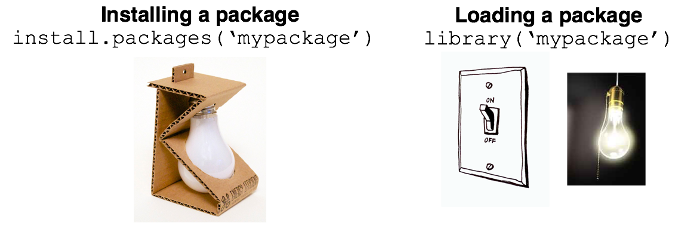
\includegraphics[width=6.89in]{images/02-package} 

}

\caption{Lamp metaphore}\label{fig:lamp}
\end{figure}

\chapter{Map creation}\label{map-creation}

\chapter{Linguistical databases}\label{db}

\section{Linguistical databases APIs}\label{api}

\section{Linguistical databases creation}\label{db-creation}

Look \ref{api} and \ref{map-creation}

\chapter{Spatial statistics}\label{statistics}

Here will be a nice sections

\chapter{Conclusion}\label{conclusion}

\bibliography{book.bib}


\end{document}
